\documentclass{article}%
\usepackage[T1]{fontenc}%
\usepackage[utf8]{inputenc}%
\usepackage{lmodern}%
\usepackage{textcomp}%
\usepackage{lastpage}%
\usepackage[head=40pt,margin=0.5in,bottom=0.6in]{geometry}%
\usepackage{graphicx}%
%
\title{\textbf{Gobierno tildó de hostil resolución del Consejo de DDHH de la ONU sobre Venezuela}}%
\author{AVN}%
\date{28/09/2018}%
%
\begin{document}%
\normalsize%
\maketitle%
\textbf{URL: }%
http://www.eluniversal.com/politica/21863/gobierno{-}tildo{-}de{-}hostil{-}resolucion{-}del{-}consejo{-}de{-}ddhh{-}de{-}la{-}onu{-}sobre{-}venezuela\newline%
%
\textbf{Periodico: }%
EU, %
ID: %
21863, %
Seccion: %
politica\newline%
%
\textbf{Palabras Claves: }%
NO\_TIENE\newline%
%
\textbf{Derecho: }%
18%
, Otros Derechos: %
5%
, Sub Derechos: %
NO\_TIENE%
\newline%
%
\textbf{EP: }%
NO\newline%
\newline%
%
\textbf{\textit{El embajador de Venezuela ante la ONU señaló que la iniciativa del Consejo de DDHH de el organismo "vulnera los principios del derecho internacional"}}%
\newline%
\newline%
%
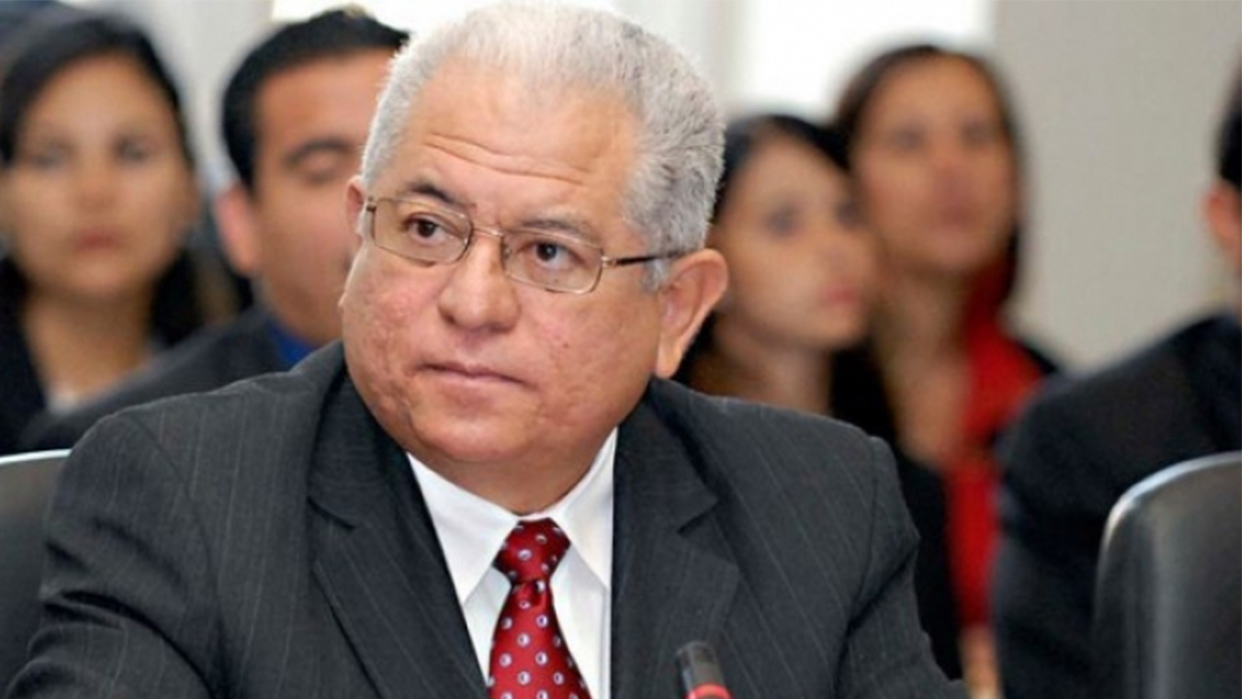
\includegraphics[width=300px]{137.jpg}%
\newline%
%
Caracas.{-}El Gobierno venezolano, en representación del ante la Organización de Naciones Unidas (ONU), Jorge Valero{-} calificó de hostil la resolución aprobada este jueves por el Consejo de Derechos Humanos de ese organismo, en la cual se insta al Ejecutivo nacional a aceptar "ayuda humanitaria" internacional para superar la crisis que vive el país.%
\newline%
%
"Rechazamos en los términos más enérgicos el proyecto de resolución. Es una iniciativa que vulnera los principios del derecho internacional, como lo son el respeto a la soberanía y la no injerencia en asuntos internos de los Estados, igualmente vulnera los pilares del multilateralismo como lo son el diálogo genuino y la cooperación", aseveró desde Ginebra, en Suiza, reseñó AVN.El diplomático señaló que la medida, impulsada por gobiernos del Grupo de Lima está sustentada en la "falsa idea" de una "crisis humanitaria", cuyo objetivo representa "el comienzo de una escalada intervencionista" para derrocar el Gobierno nacional."Los gobiernos que promueven este proyecto han declarado abiertamente que buscan remover y derrocar el Gobierno de Nicolás Maduro. Tenemos un pueblo que sufre por las medidas coercitivas unilaterales impuestas desde el exterior y que es amenazado con una intervención foránea que pretende establecer mecanismos de tutelate contra un país soberano", enfatizó.~Valero apuntó que "Venezuela es el país que más migrantes ha protegido", garantizándoles la protección de sus derechos fundamentales. En este sentido, apuntó que desde el extranjero se busca imponer "un formato que no es más que un grosero mecanismo de intervención".~Por otro lado, aseveró que la migración de venezolanos al exterior se debe a la denominada "guerra económica", que según el Gobierno, se traduce en agresiones financieras y sanciones coercitivas contra la población.~La resolución sobre Venezuela solicita a la Alta Comisionada de DDHH de la ONU, Michelle Bachelet, preparar un informe exhaustivo sobre la situación del país.~En esta línea, la también expresidenta de Chile pidió al Ejecutivo permitir la visita de una delegación de investigadores a territorio venezolano.\newline%
\newline%
Ante ello, el mandatario venezolano extendió una invitación formal a Bachelet para visitar Venezuela cuando lo considere pertinente.~Maduro indicó que la Cancillería de la República está a la orden para realizar las coordinaciones respectivas, a fin de concretar la visita.%
\newline%
%
\end{document}